% This is "sig-alternate.tex" V2.1 April 2013
% This file should be compiled with V2.5 of "sig-alternate.cls" May 2012
%
% This example file demonstrates the use of the 'sig-alternate.cls'
% V2.5 LaTeX2e document class file. It is for those submitting
% articles to ACM Conference Proceedings WHO DO NOT WISH TO
% STRICTLY ADHERE TO THE SIGS (PUBS-BOARD-ENDORSED) STYLE.
% The 'sig-alternate.cls' file will produce a similar-looking,
% albeit, 'tighter' paper resulting in, invariably, fewer pages.
%
% ----------------------------------------------------------------------------------------------------------------
% This .tex file (and associated .cls V2.5) produces:
%       1) The Permission Statement
%       2) The Conference (location) Info information
%       3) The Copyright Line with ACM data
%       4) NO page numbers
%
% as against the acm_proc_article-sp.cls file which
% DOES NOT produce 1) thru' 3) above.
%
% Using 'sig-alternate.cls' you have control, however, from within
% the source .tex file, over both the CopyrightYear
% (defaulted to 200X) and the ACM Copyright Data
% (defaulted to X-XXXXX-XX-X/XX/XX).
% e.g.
% \CopyrightYear{2007} will cause 2007 to appear in the copyright line.
% \crdata{0-12345-67-8/90/12} will cause 0-12345-67-8/90/12 to appear in the copyright line.
%
% ---------------------------------------------------------------------------------------------------------------
% This .tex source is an example which *does* use
% the .bib file (from which the .bbl file % is produced).
% REMEMBER HOWEVER: After having produced the .bbl file,
% and prior to final submission, you *NEED* to 'insert'
% your .bbl file into your source .tex file so as to provide
% ONE 'self-contained' source file.
%
% ================= IF YOU HAVE QUESTIONS =======================
% Questions regarding the SIGS styles, SIGS policies and
% procedures, Conferences etc. should be sent to
% Adrienne Griscti (griscti@acm.org)
%
% Technical questions _only_ to
% Gerald Murray (murray@hq.acm.org)
% ===============================================================
%
% For tracking purposes - this is V2.0 - May 2012

\documentclass{sig-alternate-05-2015}

\makeatletter
\def\@copyrightspace{\relax}
\makeatother 

\begin{document}

% Copyright
%\setcopyright{acmcopyright}
%\setcopyright{acmlicensed}
%\setcopyright{rightsretained}
%\setcopyright{usgov}
%\setcopyright{usgovmixed}
%\setcopyright{cagov}
%\setcopyright{cagovmixed}



\begin{comment}
% ISBN
%\isbn{123-4567-24-567/08/06}

%Conference
%\conferenceinfo{PLDI '13}{June 16--19, 2013, Seattle, WA, USA}

%\acmPrice{\$15.00}

%
% --- Author Metadata here ---
%\conferenceinfo{WOODSTOCK}{'97 El Paso, Texas USA}
%\CopyrightYear{2007} % Allows default copyright year (20XX) to be over-ridden - IF NEED BE.
%\crdata{0-12345-67-8/90/01}  % Allows default copyright data (0-89791-88-6/97/05) to be over-ridden - IF NEED BE.
% --- End of Author Metadata ---
\end{comment}
\title{Your Own Distributed System using Consensus Protocols}
\subtitle{Bellagio Casin\'o roulette multiplayer}
%
% You need the command \numberofauthors to handle the 'placement
% and alignment' of the authors beneath the title.
%
% For aesthetic reasons, we recommend 'three authors at a time'
% i.e. three 'name/affiliation blocks' be placed beneath the title.
%
% NOTE: You are NOT restricted in how many 'rows' of
% "name/affiliations" may appear. We just ask that you restrict
% the number of 'columns' to three.
%
% Because of the available 'opening page real-estate'
% we ask you to refrain from putting more than six authors
% (two rows with three columns) beneath the article title.
% More than six makes the first-page appear very cluttered indeed.
%
% Use the \alignauthor commands to handle the names
% and affiliations for an 'aesthetic maximum' of six authors.
% Add names, affiliations, addresses for
% the seventh etc. author(s) as the argument for the
% \additionalauthors command.
% These 'additional authors' will be output/set for you
% without further effort on your part as the last section in
% the body of your article BEFORE References or any Appendices.

\numberofauthors{2} %  in this sample file, there are a *total*
% of EIGHT authors. SIX appear on the 'first-page' (for formatting
% reasons) and the remaining two appear in the \additionalauthors section.
%
\author{
% You can go ahead and credit any number of authors here,
% e.g. one 'row of three' or two rows (consisting of one row of three
% and a second row of one, two or three).
%
% The command \alignauthor (no curly braces needed) should
% precede each author name, affiliation/snail-mail address and
% e-mail address. Additionally, tag each line of
% affiliation/address with \affaddr, and tag the
% e-mail address with \email.
%
% 1st. author
\alignauthor
Stefano Agostini\\
      % \affaddr{Institute for Clarity in Documentation}\\
      % \affaddr{1932 Wallamaloo Lane}\\
       %\affaddr{Wallamaloo, New Zealand}\\
       \email{agostinistefano1991@gmail.com}
\and
% 2nd. author
\alignauthor
		Salom\'e Paolo\\      
       %\affaddr{Institute for Clarity in Documentation}\\
       %\affaddr{P.O. Box 1212}\\
       %\affaddr{Dublin, Ohio 43017-6221}\\
       \email{paolosalome@gmail.com}
       \and
% 3rd. author
\alignauthor Valenti Alessandro\\
       %\affaddr{The Th{\o}rv{\"a}ld Group}\\
       %\affaddr{1 Th{\o}rv{\"a}ld Circle}\\
       %\affaddr{Hekla, Iceland}\\
       \email{alessandro.valenti1991@gmail.com}
\and
}
% There's nothing stopping you putting the seventh, eighth, etc.
% author on the opening page (as the 'third row') but we ask,
% for aesthetic reasons that you place these 'additional authors'
% in the \additional authors block, viz.
%\additionalauthors{Additional authors: John Smith (The Th{\o}rv{\"a}ld Group,
%email: {\texttt{jsmith@affiliation.org}}) and Julius P.~Kumquat
%(The Kumquat Consortium, email: {\texttt{jpkumquat@consortium.net}}).}
%\date{30 July 1999}
% Just remember to make sure that the TOTAL number of authors
% is the number that will appear on the first page PLUS the
% number that will appear in the \additionalauthors section.

\maketitle
\begin{abstract}

This paper provides a sample of a \LaTeX\ document which conforms,
somewhat loosely, to the formatting guidelines for
ACM SIG Proceedings. It is an {\em alternate} style which produces
a {\em tighter-looking} paper and was designed in response to
concerns expressed, by authors, over page-budgets.
It complements the document \textit{Author's (Alternate) Guide to
Preparing ACM SIG Proceedings Using \LaTeX$2_\epsilon$\ and Bib\TeX}.
This source file has been written with the intention of being
compiled under \LaTeX$2_\epsilon$\ and BibTeX.

The developers have tried to include every imaginable sort
of ``bells and whistles", such as a subtitle, footnotes on
title, subtitle and authors, as well as in the text, and
every optional component (e.g. Acknowledgments, Additional
Authors, Appendices), not to mention examples of
equations, theorems, tables and figures.

To make best use of this sample document, run it through \LaTeX\
and BibTeX, and compare this source code with the printed
output produced by the dvi file. A compiled PDF version
is available on the web page to help you with the
`look and feel'.
\end{abstract}


%
% The code below should be generated by the tool at
% http://dl.acm.org/ccs.cfm
% Please copy and paste the code instead of the example below. 
%
\begin{comment}

{CCSXML}
<ccs2012>
 <concept>
  <concept_id>10010520.10010553.10010562</concept_id>
  <concept_desc>Computer systems organization~Embedded systems</concept_desc>
  <concept_significance>500</concept_significance>
 </concept>
 <concept>
  <concept_id>10010520.10010575.10010755</concept_id>
  <concept_desc>Computer systems organization~Redundancy</concept_desc>
  <concept_significance>300</concept_significance>
 </concept>
 <concept>
  <concept_id>10010520.10010553.10010554</concept_id>
  <concept_desc>Computer systems organization~Robotics</concept_desc>
  <concept_significance>100</concept_significance>
 </concept>
 <concept>
  <concept_id>10003033.10003083.10003095</concept_id>
  <concept_desc>Networks~Network reliability</concept_desc>
  <concept_significance>100</concept_significance>
 </concept>
</ccs2012>  
\end{CCSXML}

\ccsdesc[500]{Computer systems organization~Embedded systems}
\ccsdesc[300]{Computer systems organization~Redundancy}
\ccsdesc{Computer systems organization~Robotics}
\ccsdesc[100]{Networks~Network reliability}


%
% End generated code
%

%
%  Use this command to print the description
%
\printccsdesc

% We no longer use \terms command
%\terms{Theory}

\keywords{ACM proceedings; \LaTeX; text tagging}
\end{comment}

\section{Introduzione}


Le tecnologie Cloud, esplose in questi ultimi anni, hanno permesso di trasferire il peso della computazione e dell'ap-provvigionamento delle risorse informatiche verso internet. Perci\'o la rete come strumento di sviluppo oggi offre scenari ampi nella direzione della distribuzione delle risorse e della computazione: la distribuzione, come nel caso che poniamo in esame, deve rappresentare un'avanguardia per lo sviluppo di applicazioni con caratteristiche di scalabilit\'a e di alta disponibilit\'a per l'utente finale. 
Gli sviluppatori utilizzando i servizi cloud possono gestire in maniera semplificata l'immagazzinamento di informazioni e l'elaborazione di molti dati, concentrandosi principalmente sullo sviluppo della loro applicazione piuttosto che nell'utilizzo di un sistema ortodosso e dispendioso come avveniva nel passato.
Aziende come \textit{Spotify}, \textit{Netflix} ed altre sfruttano il servizio cloud per rendere fruibile le loro applicazioni agli utenti di tutto il mondo, ottenendo molteplici consensi. Molti non sanno che queste applicazioni sono cos\'i efficienti proprio perch\'e sfruttano una tecnologia cloud, che per quanto possa agevolare gli utenti e gli sviluppatori, presenta sempre qualche difficolt\'a da gestire:
\begin{enumerate}
\item garantire l'accesso concorrente ad una vasta molteplicit\'a di utenti.
\item la possibilit\'a di connettersi da ogni angolo del mondo, senza ledere la qualit\'a del servizio.
\item la sincronizzazione degli eventi associati ad ogni applicativo.
\item la reperibilit\'a dei dati.
\end{enumerate}

\subsection{Obiettivi}


L'obiettivo preposto consiste nell'elaborare un gioco multiplayer che supporta molteplici entit\'a autonome che si contendono risorse condivise, l'aggiornamento in tempo reale di una qualche forma di stato condiviso, essere distribuito su molteplici nodi (eventualmente distribuiti geograficamente) e supportare la scalabilit\'a.
E' proprio con l'obiettivo di rispettare tali punti cardine che abbiamo proceduto nello sviluppo della nostra applicazione distribuita sulla piattaforma Cloud: abbiamo operato nell'intenzione di venire incontro alle esigenze degli utenti, sempre pi\'u abituati ad avere interazioni costanti e ripetute con le applicazioni di uso comune.
Il \textit{Bellagio Casin\'o} \'e l'applicazione (accessibile mediante interfaccia Web) da noi proposta che consente agli utenti di giocare ad una versione semplificata di una roulette francese condividendo un unico tavolo di gioco.
Tale applicazione permette di effettuare particolari puntate in base alla propria disponibilit\'a di credito.


\section{Architettura}


In questa sezione verr\'a illustrata a livello logico la nostra architettura descrivendo i servizi \textit{Amazon} utilizzati e i moduli sviluppati.
I componenti architetturali sono:
\begin{itemize}
\item un Cluster composto da istanze \textit{EC2 t2-micro}, situato nella regione Francoforte.
\item due Cluster composti da istanze \textit{EC2 t2-micro}, situate nella regione Eire.
\item Client.
\end{itemize}

i servizi \textit{AWS} sfruttati dai componenti sono:
\begin{itemize}
\item \textit{SNS} per la comunicazione inter-cluster.
\item \textit{DynamoDB} per la persistenza dei dati, situato nella regione Eire.
\item \textit{Redis} per supportare la logica del gioco, situato sia nella regione Eire che Francoforte.
\item \textit{LoadBalancer} per distribuire il carico dei Client. 
\end{itemize}

\begin{figure}\centering
 \includegraphics[scale=0.4]{architettura_generale} 
 \caption{Architettura} \label{nome} 
 \end{figure}
 
La motivazione che ci ha spinto nell'adottare pi\'u cluster su pi\'u aree geografiche europee \'e stata la possibilit\'a di realizzare una scalabilit\'a di tipo geografico.
Ci\'o non toglie che tale realizzazione si possa estendere anche all'interno di altre regioni geografiche messe a disposizione da \textit{AWS}. La motivazione che ci ha spinto a questa scelta \'e legata a fattori di latenza ma anche a fattori economici, oltre alla semplificazione dello sviluppo dell'applicazione e della fase di testing.




\subsection{Cluster EC2}


In questa sezione andiamo a trattare nel dettaglio quali sono le funzionalit\'a e le componenti dei Cluster \textit{EC2}.

I Cluster istanziati sono soggetti ad una gerarchia dettata dalla realizzazione di uno stato condivisibile, che corrisponde alle fasi di gioco dell'applicazione.
Pertanto possiamo suddividere tali cluster in base alla loro mansione :
\begin{itemize}
\item \textit{SuperLeader} Cluster: identifica il Cluster per la gestione dello stato di gioco, e per le azioni di registrazione e di accesso sito in Irlanda.
\item \textit{Frankfurt/Eire} Cluster: identifica uno dei Cluster di gioco sito sia in Irlanda che a Francoforte.
\end{itemize}
All'interno di ogni Cluster per mantenere lo stato corrente del gioco, abbiamo adottato \textit{Raft} come protocollo del consenso. Abbiamo utilizzato 3 istanze \textit{EC2} per Cluster, in quanto \'e il numero minimo di nodi necessario per raggiungere il consenso mediante tale protocollo.

\begin{comment}

\subsubsection{Superleader Cluster}

Tale Cluster si occupa della elaborazione dello stato corrente di gioco, e della notifica  del cambiamento di stato verso gli altri Cluster mediante il servizio SNS. 
Sfrutta il servizio offerto da DynamoDB per memorizzare i dati di registrazione dell'utente.


\subsubsection{Frankfurt/Eire Cluster}


Entrambi i Cluster svolgono le medesime attivit\'a, in quanto ricevono entrambi gli aggiornamenti dello stato attraverso il servizio di SNS.
Raccolgono le azioni di gioco prodotte dagli utenti durante le fasi di gioco, salvandole momentaneamente all'interno dell'apposita cache, la quale sfrutta il servizio Redis. 
Contattano il servizio DynamoDB per ottenere sempre i dati aggiornati dei vari giocatori, successivamente notificano al SuperLeader Cluster il completamento dell'esecuzione della fase.

\end{comment}

\section{Implementazione}
\subsection{Metodologie di sviluppo}


L'intero progetto \'e stato realizzato seguendo la metodologia di sviluppo \textit{Scrum}, la quale prevede di dividere il progetto in blocchi rapidi di lavoro(Sprint), alla fine di ciascuno dei quali si deve creare un incremento del software. L'intera stesura del progetto, dalla progettazione all'implementazione, \'e stata quindi suddivisa in sprint con scadenza molto stretta assegnati ai singoli componenti del team. 
Per la suddivisione dei task sono stati effettuati incontri giornalieri, mentre per la sincronizzazione e per il controllo di versione \'e stato utilizzato il servizio di \textit{Google Drive}. Il periodo di sviluppo, \'e stato caratterizzato da incontri giornalieri (Daily Scrum) incentrati sulla tematica del giorno, con la presenza del team al completo. A supporto dello sviluppo \'e stato previsto, fin dal primo istante, un ulteriore incontro prima della partenza di ogni nuovo sprint.La metodologia utilizzata si \'e dimostrata efficiente poich\'e ha permesso di progettare e realizzare un architettura ben congegnata in un arco temporale ridotto.
\subsection{Tecnologie utilizzate}


Il lato server del progetto \'e stato interamente realizzato utilizzando il framework \textit{Node.js}, che consente di sfruttare il linguaggio \textit{JavaScript}, tipicamente utilizzato nella client-side, anche per la scrittura di applicazioni server-side. La caratteristica principale di \textit{Node.js} risiede nella possibilit\'a di accedere alle risorse del sistema operativo in modalit\'a event-driven evitando il modello basato su processi o thread concorrenti utilizzato dai classici web server. Per facilitare l'uso di \textit{Node.js} \'e stato utilizzato il framework \textit{Express.js}, per la realizzazione semplificata del middleware \textit{HTTP}.
 L'applicazione client \'e costituita da una singola pagina \textit{HTML} con contenuti \textit{Javascript} ed elaborata attraverso l'uso della libreria \textit{JQuery} rendendo l'interfaccia dinamica, consistente e di facile utilizzo. 

\subsection{Raft}


\textit{Raft} \'e un protocollo del consenso in alternativa a \textit{Paxos} che offre la possibilit\'a di condividere uno stato comune tra i vari nodi del Cluster. Questi si suddividono in leader, candidate e follower. Viene raggiunto il consenso attraverso l'elezione di un leader, la cui mansione principale \'e quella di propagare il log dei cambiamenti di stato ai propri follower. Inoltre per ribadire la propria leadership deve informare periodicamente i propri follower attraverso dei brevi messaggi.
Ogni follower deve ricevere questi messaggi all'interno di un arco temporale fissato. Se ci\'o non dovesse avvenire verr\'a richiesta una nuova elezione di leader; colui che indice la nuova elezione cambia il proprio ruolo in candidate. Per far s\'i che \textit{Raft} tolleri \begin{math} K \end{math} guasti occorrono almeno \begin{math} 2K+1 \end{math} nodi all'interno del Cluster.

Per l'implementazione di tale protocollo \'e stato adottata la libreria \textit{Skiff}. %metterenota
 Implementa la persistenza dello stato attraverso un database \textit{in-memory} di tipo \textit{MemDown} il quale utilizza un'interfaccia \textit{LevelUp}. Per quanto concerne la comunicazione del log e dell'heartbeat utilizza server \textit{TCP}, in ascolto su ogni nodo, attraverso chiamate di tipo \textit{RPC}.
 
Le motivazioni che ci hanno condotto a questa scelta sono da addurre alla semplicit\'a di esecuzione e di condivisione del log tra i vari nodi del Cluster, la cui propagazione avviene in tempi irrisori.
L'utilizzo di \textit{Skyff} con l'architettura dei Cluster da noi ideata consente di raggiungere una certa tolleranza a guasti di vario genere sulle varie istanze \textit{EC2}.
In caso di un guasto ad una macchina, se questa risulta essere un leader quello che avviene \'e una nuova elezione, con conseguente riallineamento dei nodi del Cluster allo stato corrente del gioco.
Nel caso di un guasto nei confronti di un follower bisogna monitorare il numero di nodi presenti nel Cluster, come precedentemente illustrato.

\subsection{Comunicazione}


Per quanto riguarda la comunicazione, vogliamo porre l'attenzione verso due tipologie presenti all'interno del nostro elaborato:
\begin{itemize}
\item Comunicazione \textit{intra-Cluster}: sfruttiamo le chiamate \textit{RPC}, come descritto nel paragrafo precedente.
\item Comunicazione \textit{inter-Cluster}: Sfruttiamo il servizio \textit{AWS} di \textit{SNS}.
\end{itemize}
\textit{Amazon SNS} \'e un servizio di notifiche push rapido, flessibile e completamente gestito che ti consente di inviare messaggi individuali o collettivi a un numero elevato di destinatari. Grazie a questa soluzione, inviare notifiche push a utenti di dispositivi mobili, destinatari di posta o addirittura altri servizi distribuiti \'e semplice e conveniente.
Per comunicare lo stato del gioco a tutti nodi dei vari Cluster sono stati creati 5 \textit{Topic} per permettere lo scambio di informazioni e di cambiamento di stato, ci\'o verr\'a chiarificato successivamente.

La motivazione per cui \'e stato scelto questo servizio sono le seguenti:
\begin{itemize}
\item \textit{SNS} permette la realizzazione di un servizio di tipo \textit{Publish/Subscribe}.
\item Sfrutta endpoint di tipo \textit{http} per la ricezione di notifiche.
\item Permette la comunicazione tra pi\'u aree geografiche.
\item Garantisce un certo grado di riservatezza.
\end{itemize}
Generalmente \textit{SNS} viene utilizzato in abbinamento con \textit{SQS}, per\'o nel nostro caso non avevamo una necessit\'a di permanenza e di ordinamento dei messaggi.

\subsection{Persistenza}


Poich\'e la nostra applicazione \'e un gioco multiplayer e avendo necessit\'a di gestire la registrazione e l'accesso di pi\'u giocatori, ci occorre un servizio di persistenza dati. A tal proposito la persistenza \'e stata realizzata sfruttando due tipi di servizio:
\begin{itemize}
\item \textit{Redis}: \'e un servizio di cache distribuito di \textit{Amazon AWS}.
\item \textit{DynamoDB}:  \'e un database \textit{NoSQL} distribuito di \textit{Amazon AWS}.
\end{itemize}

Nel dettaglio \textit{Redis} viene sfruttato dai Cluster di gioco per poter immagazzinare le ultime informazioni relative alle puntate degli utenti, rendendo tali dati accessibili per l'elabo-razione delle vincite da parte del sistema. Alla fine di questa operazione il sistema provveder\'a all'eliminazione di tali dati per permettere l'aggiornamento degli stessi coerentemente con la mano del gioco.

Per quanto concerne \textit{DynamoDB} sono state create due tabelle
\begin{itemize}
\item  una per conservare i dati relativi agli utenti (credenziali di accesso e credito).
\item  una per conservare le puntate elaborate dal sistema, precedentemente contrassegnate come vincenti o perdenti.
\end{itemize}
Quando un'applicazione effettua delle scritture su una tabella in \textit{DynamoDB} i dati impiegano del tempo per propagarsi in ogni locazione di memoria della regione \textit{AWS} corrente. I dati saranno consistenti in tutte le locazioni di memoria in un periodo lungo \begin{math}\sim{~1}\end{math} sec o anche meno.
Dato che la nostra applicazione non effettua chiamate al Database frequentemente, la scelta dell'\textit{eventual consistency} ci \'e sembrata la pi\'u opportuna anche in termini di costi.

Abbiamo sfruttato la \textit{chiave di partizionamento} che offre \textit{DynamoDB} per collocare tramite funzione hash le puntate appartenenti alla stessa mano nella stessa partizione; cos\'i come la \textit{chiave di ordinamento} per catalogare nella stessa partizione le puntate appartenenti ad utenti differenti.
Su consiglio delle linee guida fornite da \textit{DynamoDB} abbiamo scelto di utilizzare come chiave di partizionamento la \textit{mano} del gioco poich\'e offre un range di valori pi\'u ampio rispetto a quello offerto dalla chiave \textit{username}. 

\begin{figure}\centering
 \includegraphics[scale=0.5]{Database} 
 \caption{Processo scrittura delle puntate con interazione DynamoDB e Redis} \label{nome} 
 \end{figure}
 
\subsection{Implementazione Clusters}


Come illustrato precedentemente i Cluster da noi sviluppati possono essere suddivisi funzionalmente in due gruppi distinti: \textit{SuperLeader} e \textit{Frankfurt/Eire} Cluster.
Tutti i Cluster definiti sono configurati, come precedentemente indicato nella sezione Architettura, con un numero fissato pari a 3 di istanze \textit{EC2}.
La scelta di tale numero permette la gestione di un solo guasto (come descritto in \textit{Raft}) e aumentando il numero di istanze il risultato sarebbe invariato con un grado di tolleranza ai guasti maggiore.
Un'altra motivazione che ci ha spinto a tale scelta \'e di natura economica.
In ogni caso l'aggiunta o meno di altre istanze all'interno dei nostri Cluster pu\'o essere effettuata senza alcun problema, a patto che vengano identificate all'interno di una \textit{VPC} attraverso un tag univoco. Il sistema \'e configurato in modo che ogni istanza all'avvio sappia identificare esattamente quali sono le macchine appartenenti al proprio gruppo, permettendole di sfruttare il protocollo \textit{Raft} per comunicare con tutte le entit\'a del proprio gruppo.
Tutto ci\'o sinteticamente rappresenta un servizio di \textit{Discovery Service} atto a configurare dinamicamente i Cluster \textit{Raft}.

\subsubsection{Stati del Sistema}


Poniamo ora l'attenzione verso gli Stati del Sistema.
I due tipi di stato che si alternano sono:
\begin{itemize}
\item \textit{Play}: identifica le fasi di gioco dell'applicazione in cui l'utente pu\'o effettuare la puntata desiderata.
\item \textit{Compute}: identifica la fase di estrazione del numero e il calcolo delle puntate vincenti.
\end{itemize}
Nella definizione di questi stati viene allegato l'istante di tempo in cui viene generato.
Si ha un cambiamento di stato quando entrambi i Cluster di gioco comunicano la terminazione dello stato corrente, come illustrato nella figura ~\ref{fig:stateSystem}.

\begin{figure}\centering
 \includegraphics[scale=0.4]{Stati_del_sistema} 
 \caption{Rappresentazione degli Stati del sistema} 
\label{fig:stateSystem}
 \end{figure}

\subsubsection{SuperLeader}


Il \textit{SuperLeader} \'e il Cluster adibito alla definizione dello stato di gioco e all'accesso e alla registrazione degli utenti.

Come primo passo definiamo la gerarchia del Cluster che si compone di un leader e di due peer(follower).
Tale definizione \'e derivata dai ruoli che impone \textit{Raft}.
Il leader, cos\'i come i due peer, si compone di due processi :
\begin{itemize}
\item processo Raft (padre) che si occupa del consenso per mezzo di server \textit{TCP} e sfrutta \textit{SNS} per pubblicare i cambi di stato.
\item processo \textit{HTTP} (figlio) che si occupa di ricevere le notifiche \textit{SNS} e le richieste da parte degli utenti.
\end{itemize}

Il processo \textit{Raft} sfrutta la libreria \textit{Skiff} per mantenere il consenso su un determinato stato di gioco attraverso la propagazione del log e mediante chiamate \textit{RPC}.
Nella fase di inizializzazione il leader si sottoscrive ai topic di interesse:
\begin{itemize}
\item \textit{Computed}: su questo topic attende i messaggi che indicano la conclusione della fase di gioco \textit{Compute} da parte dei Cluster di gioco. Una volta ricevuti i messaggi da entrambi effettua la transizione di stato \textit{Compute} $\rightarrow$ \textit{Play} e lo invia ai Cluster di gioco. 
\item \textit{Played}: su questo topic attende i messaggi che indicano la conclusione della fase di gioco \textit{Play} da parte dei Cluster di gioco. Una volta ricevuti i messaggi da entrambi effettua la transizione di stato \textit{Play} $\rightarrow$  \textit{Compute},  genera il numero della Roulette inserendolo nello stato per poi inviare quest'ultimo ai Cluster di gioco.
\end{itemize}

Lo schema soprastante rappresenta il ciclo naturale di esecuzione del leader. In caso di guasto di quest'ultimo viene innescata una procedura di rientro che coinvolge il nuovo leader. Esso:
\begin{itemize}
\item si sottoscrive al topic \textit{LeaderState}.
\item richiede ad entrambi i Cluster di gioco il loro stato corrente, i quali a loro volta lo pubblicheranno sul topic \textit{LeaderState}.
\item confronta lo stato ricevuto da ognuno dei Custer con il suo stato corrente e se il primo \'e pi\'u recente rispetto al secondo lo sostituisce.
\item si sottoscrive ai topic \textit{Computed} e \textit{Played} e successivamente chiede ai Cluster di gioco di ritrasmettere l'ultima azione (\textit{Computed} o \textit{Played}) da loro completata.
\item riprende la normale esecuzione descritta sopra.
\end{itemize} 

A differenza di questa funzione legata alla generazione degli stati del sistema, associata unicamente al leader, qualsiasi nodo del Cluster \textit{SuperLeader} si occupa della registrazione e dell'accesso di nuovi utenti. Attraverso la pagina web messa a disposizione agli utenti, questi possono effettuare la propria sottoscrizione al gioco: 
\begin{itemize}
\item la richiesta \textit{HTTP} viene catturata dal \textit{middleware Express} del nodo server contattato.
\item vengono estratte le credenziali dell'utente, e rese persistenti sulla tabella \textit{Accounts} per mezzo delle \textit{DynamoApi}.
\item viene inviato al \textit{client HTTP} la conferma di avvenuta registrazione.
\end{itemize}
Per quanto riguarda il login degli utenti, il nodo del Cluster contattato alla ricezione di una tale richiesta:
\begin{itemize}
\item cattura la richiesta \textit{HTTP} e ne estrae le credenziali tramite \textit{middleware Express}.
\item controlla che le credenziali siano presenti nella tabella \textit{Accounts} di \textit{DynamoDB}.
\end{itemize}



\subsubsection{Frankfurt/Eire Cluster}


I Cluster di gioco si occupano dell'esecuzione delle operazioni relative allo stato corrente del sistema. Essi operano in due regioni differenti ma sono esattamente equivalenti, pertanto ne illustreremo soltanto uno. 

Il Cluster di gioco sfrutta le funzionalit\'a offerte da \textit{Skiff} per mantenere il consenso sullo stato corrente tra i suoi nodi mediante chiamate \textit{RPC} e per crearne una gerarchia (\textit{follower/leader}).
Il leader, cos\'i come i due peer, si compone di due processi :
\begin{itemize}
\item processo Raft (padre) che si occupa del consenso per mezzo di server \textit{TCP} e sfrutta \textit{SNS} per pubblicare la terminazione della fase corrente di gioco (\textit{Computed / Played}).
\item processo \textit{HTTP} (figlio) che si occupa di ricevere le notifiche \textit{SNS} e le richieste da parte degli utenti.
\end{itemize}

Nella fase di inizializzazione il leader si sottoscrive al topic di interesse \textit{RegionLeaderTopic}. Su questo topic attende notifiche da parte del Cluster \textit{SuperLeader} che si differenziano in funzione del contenuto:
\begin{itemize}
\item se il contenuto \'e un \textit{JSON} allora identifica un nuovo stato del sistema, al quale il Cluster di gioco dovr\'a allinearsi ed eseguire le relative operazioni.
\item se il contenuto \'e la stringa \textit{currentState} allora identifica la richiesta dello stato corrente del Cluster di gioco. Questa notifica viene inviata dal leader del Cluster \textit{SuperLeader} quando \'e stata innescata la procedura di rientro di quest'ultimo.
\item se il contenuto \'e la stringa \textit{lastMessage} allora identifica la richiesta di ritrasmissione dell'ultimo messaggio di terminazione fase inviato (\textit{Computed / Played}). Questa notifica viene inviata dal leader del Cluster \textit{SuperLeader} quando viene innescata la procedura di rientro di quest'ultimo.
\end{itemize} 

Di conseguenza alla ricezione della notifica di cambio di stato del sistema nel nodo leader possono verificarsi due scenari differenti:
\begin{itemize}
\item il valore del campo \textit{phase} dello stato ricevuto corrisponde a \textit{Play}. Il leader del Cluster di gioco crea un processo che gestisce la nuova fase. Per un tempo pari a \textit{20 secondi} quest'ultimo permane nello stato \textit{Play}, terminato il quale pubblica sul topic \textit{Played} il suo completamento specificando la sua zona di appartenenza (\textit{Frankfurt o Eire}); infine aggiorna nel db \textit{in-memory di Skiff} il valore identificato dalla chiave \textit{lastMessage} al valore \textit{Played}.
In questa fase, inoltre, ogni nodo del Cluster di gioco (sincronizzato mediante \textit{Skiff} allo stato \textit{Play} corrente) riceve dai client connessi le puntate effettuate dagli utenti e le salva di conseguenza all'interno della cache \textit{Redis} della regione in questione.  
\item il valore del campo \textit{phase} dello stato ricevuto corrisponde a \textit{Compute}. Il leader del Cluster di gioco crea un processo che gestisce la nuova fase. Per un tempo pari a \textit{8 secondi} quest'ultimo permane nello stato \textit{Compute}, terminato il quale pubblica sul topic \textit{Computed} il suo completamento specificando la sua zona di appartenenza (\textit{Frankfurt o Eire}); infine aggiorna nel db \textit{in-memory di Skiff} il valore identificato dalla chiave \textit{lastMessage} al valore \textit{Computed}.
Durante quest'arco temporale il leader del Cluster di gioco preleva dalla cache \textit{Redis} le puntate raccolte durante la fase precedente, ne calcola l'esito e le salva sulla tabella \textit{Bets} di \textit{DynamoDB}. Dopodich\'e aggiorna il credito di ogni utente che ha effettuato la puntata all'interno della tabella \textit{Accounts} ed infine libera la cache per la nuova fase.
\end{itemize}

Lo schema soprastante rappresenta il ciclo naturale di esecuzione del leader. In caso di guasto di quest'ultimo viene innescata una procedura di rientro che coinvolge il nuovo leader. Prima di effettuarla il nuovo leader provveder\'a ad effettuare le sottoscrizioni descritte prima. In base allo stato di \textit{Skiff} che ha ereditato adotta due comportamenti differenti:
\begin{itemize}
\item se la sua fase corrisponde a \textit{Play} allora il leader calcola il tempo di gioco restante rispetto all'istante di inizio della fase (lo stato ha come attributo un \textit{timestamp} di creazione stato) al termine del quale comunica al \textit{SuperLeader} la terminazione della fase; infine riprende la normale procedura di esecuzione precedentemente descritta. 
\item se la sua fase corrisponde a \textit{Compute} allora il leader cerca eventuali puntate nella cache e, se presenti, le elabora calcolandone l'esito e le salva nella tabella \textit{Bets}; di conseguenza comunica al \textit{SuperLeader} la terminazione della fase e riprende la normale esecuzione. 
\end{itemize}

\subsection{Bilanciamento del carico}


Per bilanciare il carico dei client su tutti i nodi presenti nei Cluster abbiamo deciso di utilizzare il servizio di Amazon \textit{Application Load Balancer}. Il servizio garantisce anche un'analisi sempre aggiornata dello stato di salute dei nodi del Cluster iscritti, inoltrando le richieste Client solo alle istanze \textit{healty}.
Ci occorreva un servizio semplice e configurabile dinamicamente che permettesse di rendere il sistema bilanciato rispetto al numero di Client indipendentemente dal numero di istanze \textit{EC2} del Cluster. L'utilizzo di tale servizio rallenta il processo di saturazione delle risorse poich\'e impedisce una concentrazione eccessiva di connessioni su uno stesso nodo. Tutto ci\'o contribuisce a rendere il sistema pi\'u robusto e meno esposto a guasti.

Abbiamo configurato tre \textit{Load Balancer} di cui due per i Cluster della regione \textit{Irlanda} e uno per il Cluster della regione \textit{Francoforte}. Inoltre abbiamo sfruttato il \textit{Cookie Stickiness} il quale permette di mantenere la connessione \textit{Client \ Server} stabile su una sola macchina per un intervallo di tempo fissato (nel nostro caso \textit{3 secondi}); questo risulta utile nei casi in cui un server target sta diventanto \textit{unhealty} ma non risulta ancora tale per il \textit{Load Balancer}.   

\subsection{Scalabilit\'a}
Il termine scalabilit\'a, nelle telecomunicazioni, nell'ingegneria del software, in informatica e in altre discipline, si riferisce, in termini generali, alla capacit\'a di un sistema di "crescere" o diminuire di scala in funzione delle necessit\'a e delle disponibilit\'a. Un sistema che gode di questa propriet\'a viene detto scalabile.
La tipologia di scalabilit\'a implementata nel nostro sistema \'e quella \textit{geografica}.
Un sistema geograficamente scalabile \'e quello che mantiene inalterata la sua usabilit\'a e utilit\'a indipendentemente dalla distanza fisica dei suoi utenti o delle sue risorse.

Poich\'e il nostro sistema viene installato all'interno di pi\'u nodi situati in diverse aree geografiche, abbiamo analizzato varie \textit{policy} che permettessero una gestione dinamica del carico degli utenti sui nodi della rete, mantenendo un servizio efficiente indipendentemente dalla propria distanza dal Cluster. A tal proposito abbiamo sfruttato le funzionalit\'a offerte dal servizio \textit{AWS Load Balancer} per distribuire il carico sui vari nodi, come illustrato in precedenza, ed \'e stata adottata una politica di \textit{Ping} per il reindirizzamento dell'utente al Cluster, permettendogli di accedere alle risorse senza avere una grossa latenza.
Sfruttando tale \textit{policy} implementiamo la scalabilit\'a geografica all'interno del protocollo di rete:
\begin{enumerate}
\item Si effettua il ping verso gli indirizzi dei due \textit{Load Balancer} siti in due aree geografiche distinte.
\item Si analizza il \textit{RTT} prodotto ricercando il minore tra i due.
\item Si reindirizza l'utente verso il \textit{Load Balancer} che ha generato il \textit{RTT} minore.
\end{enumerate}
 
Non sfruttiamo \textit{policy} come la localizzazione dell'indirizzo \textit{IP} in quanto risulta essere sconveniente per effettuare una connessione ad una regione piuttosto che ad un'altra, poich\'e non sempre la ridotta distanza fisica (distanza tra la macchina usata dall'utente ed il server ospitante il \textit{Load Balancer}) rispecchia una vicinanza in termini di rete.

Tale procedura \'e implementata nel Client del Cluster \textit{SuperLeader} e viene innescata in corrispondenza del login di un utente alla piattaforma di gioco. In questo modo il Cluster distribuisce gli utenti sui diversi Cluster di gioco.

\subsection{Client}

Per l'elaborazione della piattaforma di gioco \'e stata implementata una singola pagina \textit{HTML} che sfrutta  i servizi offerti da \textit{Bootstrap}, \textit{CSS}, ed infine \textit{JQuery} per la logica dietro la pagina.
Prima di trattare la logica implementativa, poniamo l'attenzione sulle fasi del gioco presenti all'interno dell'applicazione.
Le fasi di gioco sono 4 e servono per identificare le varie fasi dettate dal gioco della roulette.
\begin{itemize}
\item \textit{Place your bet}: in questa fase ogni utente che abbia effettuato l'accesso alla piattaforma ha a disposizione $\sim{~}$15 secondi per puntare sulla roulette.
\item \textit{Last bets}: in questa fase ogni utente che abbia effettuato l'accesso alla piattaforma ha a disposizione gli ultimi $\sim{~}$5 secondi per puntare sulla roulette.
\item \textit{No more bets}: in questa fase l'utente non pu\'o pi\'u effettuare puntate mentre attende l'uscita del numero del turno.
\item \textit{Payment}: in caso di vincita si effettua l'aggiornamento del credito a disposizione dell'utente.
\end{itemize}

Queste fasi di gioco del Client corrispondono alle fasi dettate dalle regole di gioco della roulette, ed inoltre vengono utilizzate per effettuare la sincronizzazione con le fasi del Server.
A tal proposito le prime due fasi, \textit{Place your bet} e \textit{Last Bets} corrispondono alla fase di \textit{Play} definita nel server, descritta nei paragrafi precedenti. La durata di queste due fasi \'e pensata in modo che ci sia una sincronia con le fasi del server, evitando cos\'i che le puntate degli utenti vengano effettuate durante la fase errata. Le restanti fasi, \textit{No more bets} e \textit{Payment}, corrispondono alla fase di \textit{Compute} del server. Durante queste ultime fasi vengono effettuate diverse chiamate rest verso il \textit{Load Balancer}, il quale contatter\'a a sua volta  i nodi ad esso registrati, ricevendo le informazioni richieste, tra cui il credito dell'utente e lo stato del gioco.
La fase di \textit{Payment}, oltre alla funzione descritta in precedenza, svolge una funzione aggiuntiva di riallineamento con lo stato del server, quando necessaria, in caso di guasto di quest'ultimo.(vedi figure~\ref{fig:clientState}).
 \begin{figure}\centering
 \includegraphics[scale=0.5]{stati_client} 
 \caption{Rappresentazione degli Stati del Client} 
\label{fig:clientState}
 \end{figure}

\subsection{Esempio Flusso di Esecuzione}
Qui di seguito illustriamo la tipica esecuzione di un utente che vuole entrare nella piattaforma per iniziare a giocare:
\begin{itemize}
\item Contatta l'\textit{indirizzo DNS} del \textit{Load Balancer} relativo al Cluster \textit{SuperLeader} e questo risponde fornendo la pagina di login.
\item Una volta richiesto l'accesso attraverso il form dedicato viene mandata un ulteriore richiesta al \textit{Load Balancer} per confermare le credenziali. 
\item Il \textit{Load Balancer} rimanda la richiesta ad uno dei server del Cluster \textit{SuperLeader} il quale controlla le credenziali; una volta confermate si "pingano" gli altri \textit{Load Balancer} e si seleziona quello con il \textit{RTT} minore.
\item Viene instradata la richiesta verso il \textit{Load Balancer} della regione cos\'i selezionata il quale fornisce la pagina di gioco.
\item Al primo accesso dell'utente alla piattaforma di gioco assegnata gli verr\'a richiesta la conferma di un codice di accesso (\textit{daily code}). Se il codice \'e corretto si accede alla piattaforma altrimenti si ritorna alla pagina di login.
\end{itemize}

\section{Test}
In data 25/11/2016 dalle ore 14:30 alle ore 17:30 abbiamo testato il nostro sistema coinvolgendo colleghi dell'ambiente universitario. Lo scopo principale del test \'e stato monitorare la capacit\'a di adattamento del sistema alle variazioni del carico e l'efficacia della \textit{policy del ping} per il processo di \textit{redirect}. 

Il campione di utenti era costituito prevalentemente da utenti di nazionalit\'a italiana con l'eccezione di un utente residente a Londra ed un secondo residente a Siviglia.  Entrambi hanno osservato che il server di gioco al quale si sono collegati era appartenente al Cluster irlandese; ci\'o indica che il \textit{RTT} del \textit{ping} \'e anche influenzato dalla distanza geografica delle entit\'a comunicanti oltre che dalla distanza in termini di rete, non tradendo le nostre aspettative. Tutti gli altri utenti, situati nel territorio nazionale, hanno sperimentato un reindirizzameto al Cluster della regione geografica di Francoforte.

Durante il test si sono registrati e connessi ai server di gioco 30 utenti distribuiti durante l'arco temporale sopra indicato. Per mezzo del servizio \textit{Cloud Watch} abbiamo prelevato dei dati riguardanti l'andamento del carico dei tre \textit{Load Balancer}. Le metriche riportate sui grafici riguardano i valori medi in un intervallo di \textit{5 minuti} delle connessioni attive e di quelle in ingresso. 

 \begin{figure}
 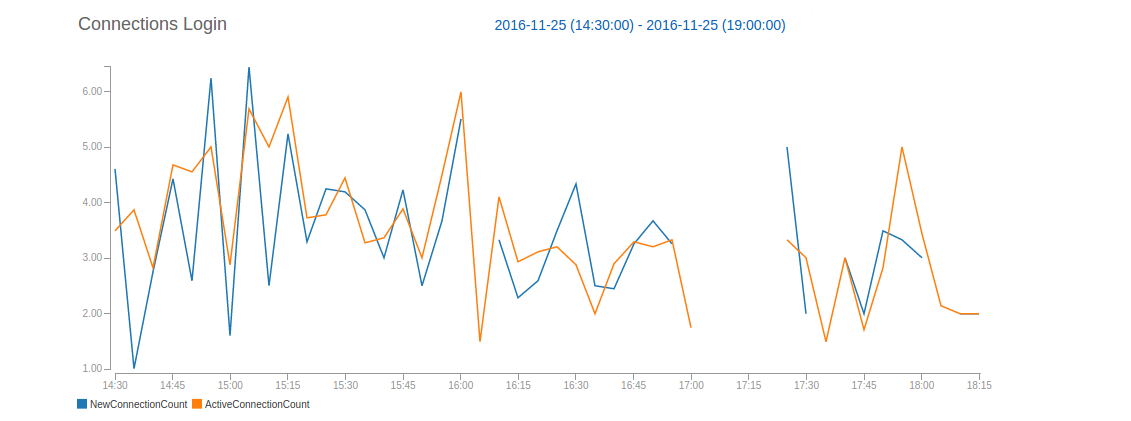
\includegraphics[scale=0.35]{connection_login} 
 \caption{Andamento delle metriche del \textit{Load Balancer del SuperLeader}} 
\label{fig:connectionLogin}
 \end{figure}

 
\section{Sviluppi Futuri}

\section{Conclusioni}


\subsection{Type Changes and {\subsecit Special} Characters}1
We have already seen several typeface changes in this sample.  You
can indicate italicized words or phrases in your text with
the command \texttt{{\char'134}textit}; emboldening with the
command \texttt{{\char'134}textbf}
and typewriter-style (for instance, for computer code) with
\texttt{{\char'134}texttt}.  But remember, you do not
have to indicate typestyle changes when such changes are
part of the \textit{structural} elements of your
article; for instance, the heading of this subsection will
be in a sans serif\footnote{A third footnote, here.
Let's make this a rather short one to
see how it looks.} typeface, but that is handled by the
document class file. Take care with the use
of\footnote{A fourth, and last, footnote.}
the curly braces in typeface changes; they mark
the beginning and end of
the text that is to be in the different typeface.

You can use whatever symbols, accented characters, or
non-English characters you need anywhere in your document;
you can find a complete list of what is
available in the \textit{\LaTeX\
User's Guide}\cite{Lamport:LaTeX}.

\subsection{Math Equations}
You may want to display math equations in three distinct styles:
inline, numbered or non-numbered display.  Each of
the three are discussed in the next sections.

\subsubsection{Inline (In-text) Equations}
A formula that appears in the running text is called an
inline or in-text formula.  It is produced by the
\textbf{math} environment, which can be
invoked with the usual \texttt{{\char'134}begin. . .{\char'134}end}
construction or with the short form \texttt{\$. . .\$}. You
can use any of the symbols and structures,
from $\alpha$ to $\omega$, available in
\LaTeX\cite{Lamport:LaTeX}; this section will simply show a
few examples of in-text equations in context. Notice how
this equation: \begin{math}\lim_{n\rightarrow \infty}x=0\end{math},
set here in in-line math style, looks slightly different when
set in display style.  (See next section).

\subsubsection{Display Equations}
A numbered display equation -- one set off by vertical space
from the text and centered horizontally -- is produced
by the \textbf{equation} environment. An unnumbered display
equation is produced by the \textbf{displaymath} environment.

Again, in either environment, you can use any of the symbols
and structures available in \LaTeX; this section will just
give a couple of examples of display equations in context.
First, consider the equation, shown as an inline equation above:
\begin{equation}\lim_{n\rightarrow \infty}x=0\end{equation}
Notice how it is formatted somewhat differently in
the \textbf{displaymath}
environment.  Now, we'll enter an unnumbered equation:
\begin{displaymath}\sum_{i=0}^{\infty} x + 1\end{displaymath}
and follow it with another numbered equation:
\begin{equation}\sum_{i=0}^{\infty}x_i=\int_{0}^{\pi+2} f\end{equation}
just to demonstrate \LaTeX's able handling of numbering.

\subsection{Citations}
Citations to articles \cite{bowman:reasoning,
clark:pct, braams:babel, herlihy:methodology},
conference proceedings \cite{clark:pct} or
books \cite{salas:calculus, Lamport:LaTeX} listed
in the Bibliography section of your
article will occur throughout the text of your article.
You should use BibTeX to automatically produce this bibliography;
you simply need to insert one of several citation commands with
a key of the item cited in the proper location in
the \texttt{.tex} file \cite{Lamport:LaTeX}.
The key is a short reference you invent to uniquely
identify each work; in this sample document, the key is
the first author's surname and a
word from the title.  This identifying key is included
with each item in the \texttt{.bib} file for your article.

The details of the construction of the \texttt{.bib} file
are beyond the scope of this sample document, but more
information can be found in the \textit{Author's Guide},
and exhaustive details in the \textit{\LaTeX\ User's
Guide}\cite{Lamport:LaTeX}.

This article shows only the plainest form
of the citation command, using \texttt{{\char'134}cite}.
This is what is stipulated in the SIGS style specifications.
No other citation format is endorsed or supported.

\subsection{Tables}
Because tables cannot be split across pages, the best
placement for them is typically the top of the page
nearest their initial cite.  To
ensure this proper ``floating'' placement of tables, use the
environment \textbf{table} to enclose the table's contents and
the table caption.  The contents of the table itself must go
in the \textbf{tabular} environment, to
be aligned properly in rows and columns, with the desired
horizontal and vertical rules.  Again, detailed instructions
on \textbf{tabular} material
is found in the \textit{\LaTeX\ User's Guide}.

Immediately following this sentence is the point at which
Table 1 is included in the input file; compare the
placement of the table here with the table in the printed
dvi output of this document.

\begin{table}
\centering
\caption{Frequency of Special Characters}
\begin{tabular}{|c|c|l|} \hline
Non-English or Math&Frequency&Comments\\ \hline
\O & 1 in 1,000& For Swedish names\\ \hline
$\pi$ & 1 in 5& Common in math\\ \hline
\$ & 4 in 5 & Used in business\\ \hline
$\Psi^2_1$ & 1 in 40,000& Unexplained usage\\
\hline\end{tabular}
\end{table}

To set a wider table, which takes up the whole width of
the page's live area, use the environment
\textbf{table*} to enclose the table's contents and
the table caption.  As with a single-column table, this wide
table will ``float" to a location deemed more desirable.
Immediately following this sentence is the point at which
Table 2 is included in the input file; again, it is
instructive to compare the placement of the
table here with the table in the printed dvi
output of this document.


\begin{table*}
\centering
\caption{Some Typical Commands}
\begin{tabular}{|c|c|l|} \hline
Command&A Number&Comments\\ \hline
\texttt{{\char'134}alignauthor} & 100& Author alignment\\ \hline
\texttt{{\char'134}numberofauthors}& 200& Author enumeration\\ \hline
\texttt{{\char'134}table}& 300 & For tables\\ \hline
\texttt{{\char'134}table*}& 400& For wider tables\\ \hline\end{tabular}
\end{table*}
% end the environment with {table*}, NOTE not {table}!

\subsection{Figures}
Like tables, figures cannot be split across pages; the
best placement for them
is typically the top or the bottom of the page nearest
their initial cite.  To ensure this proper ``floating'' placement
of figures, use the environment
\textbf{figure} to enclose the figure and its caption.

This sample document contains examples of \textbf{.eps} files to be
displayable with \LaTeX.  If you work with pdf\LaTeX, use files in the
\textbf{.pdf} format.  Note that most modern \TeX\ system will convert
\textbf{.eps} to \textbf{.pdf} for you on the fly.  More details on
each of these is found in the \textit{Author's Guide}.

\begin{figure}
\centering
%
\includegraphics{fly}
\caption{A sample black and white graphic.}
\end{figure}

\begin{figure}
\centering
%
\includegraphics[height=1in, width=1in]{fly}
\caption{A sample black and white graphic
that has been resized with the \texttt{includegraphics} command.}
\end{figure}


As was the case with tables, you may want a figure
that spans two columns.  To do this, and still to
ensure proper ``floating'' placement of tables, use the environment
\textbf{figure*} to enclose the figure and its caption.
and don't forget to end the environment with
{figure*}, not {figure}!

\begin{figure*}
\centering
%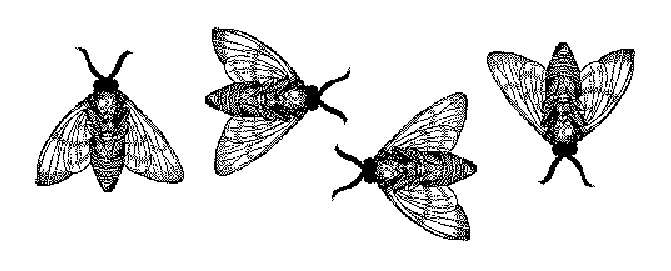
\includegraphics{flies}
\caption{A sample black and white graphic
that needs to span two columns of text.}
\end{figure*}


\begin{figure}
\centering
%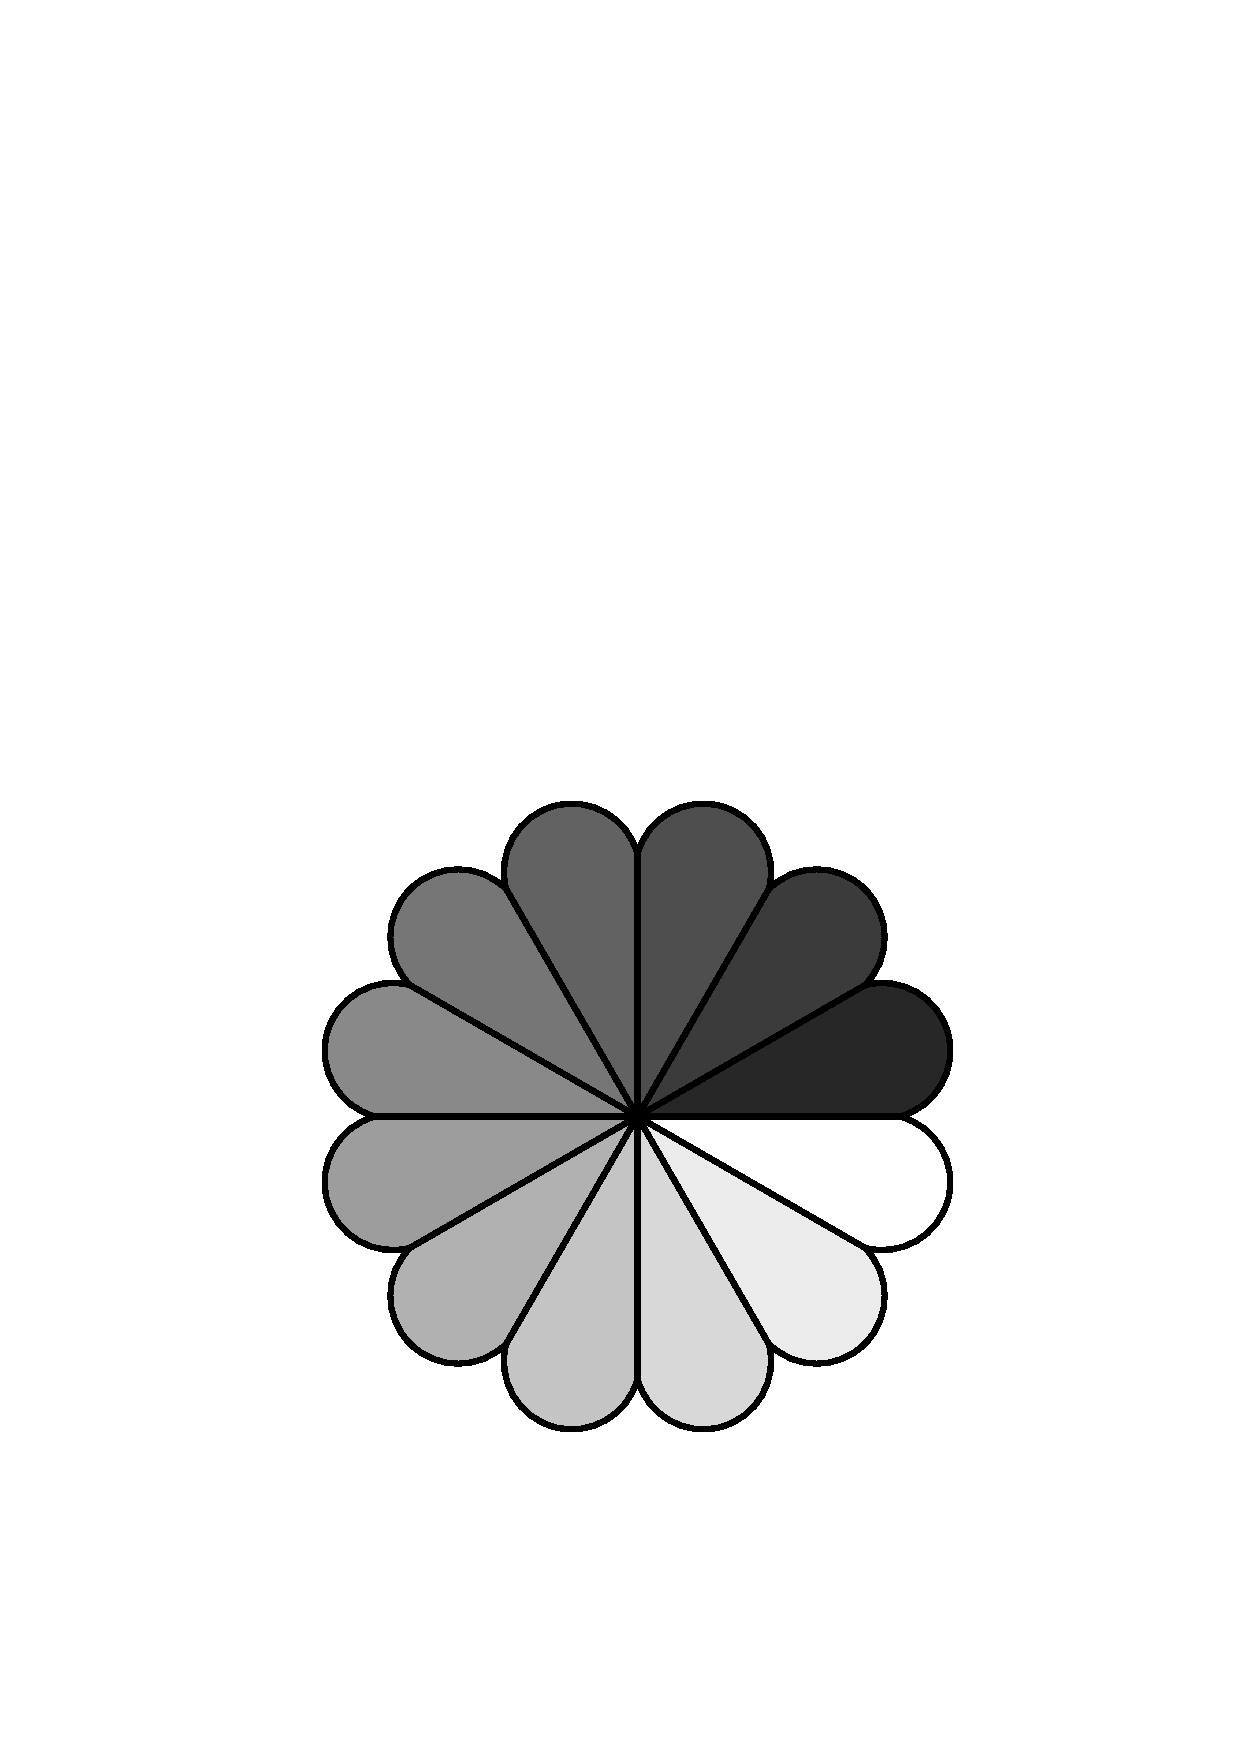
\includegraphics[height=1in, width=1in]{rosette}
\caption{A sample black and white graphic that has
been resized with the \texttt{includegraphics} command.}
\vskip -6pt
\end{figure}

\subsection{Theorem-like Constructs}
Other common constructs that may occur in your article are
the forms for logical constructs like theorems, axioms,
corollaries and proofs.  There are
two forms, one produced by the
command \texttt{{\char'134}newtheorem} and the
other by the command \texttt{{\char'134}newdef}; perhaps
the clearest and easiest way to distinguish them is
to compare the two in the output of this sample document:

This uses the \textbf{theorem} environment, created by
the\linebreak\texttt{{\char'134}newtheorem} command:
\newtheorem{theorem}{Theorem}
\begin{theorem}
Let $f$ be continuous on $[a,b]$.  If $G$ is
an antiderivative for $f$ on $[a,b]$, then
\begin{displaymath}\int^b_af(t)dt = G(b) - G(a).\end{displaymath}
\end{theorem}

The other uses the \textbf{definition} environment, created
by the \texttt{{\char'134}newdef} command:
\newdef{definition}{Definition}
\begin{definition}
If $z$ is irrational, then by $e^z$ we mean the
unique number which has
logarithm $z$: \begin{displaymath}{\log e^z = z}\end{displaymath}
\end{definition}

Two lists of constructs that use one of these
forms is given in the
\textit{Author's  Guidelines}.
 
There is one other similar construct environment, which is
already set up
for you; i.e. you must \textit{not} use
a \texttt{{\char'134}newdef} command to
create it: the \textbf{proof} environment.  Here
is a example of its use:
\begin{proof}
Suppose on the contrary there exists a real number $L$ such that
\begin{displaymath}
\lim_{x\rightarrow\infty} \frac{f(x)}{g(x)} = L.
\end{displaymath}
Then
\begin{displaymath}
l=\lim_{x\rightarrow c} f(x)
= \lim_{x\rightarrow c}
\left[ g{x} \cdot \frac{f(x)}{g(x)} \right ]
= \lim_{x\rightarrow c} g(x) \cdot \lim_{x\rightarrow c}
\frac{f(x)}{g(x)} = 0\cdot L = 0,
\end{displaymath}
which contradicts our assumption that $l\neq 0$.
\end{proof}

Complete rules about using these environments and using the
two different creation commands are in the
\textit{Author's Guide}; please consult it for more
detailed instructions.  If you need to use another construct,
not listed therein, which you want to have the same
formatting as the Theorem
or the Definition\cite{salas:calculus} shown above,
use the \texttt{{\char'134}newtheorem} or the
\texttt{{\char'134}newdef} command,
respectively, to create it.

\subsection*{A {\secit Caveat} for the \TeX\ Expert}
Because you have just been given permission to
use the \texttt{{\char'134}newdef} command to create a
new form, you might think you can
use \TeX's \texttt{{\char'134}def} to create a
new command: \textit{Please refrain from doing this!}
Remember that your \LaTeX\ source code is primarily intended
to create camera-ready copy, but may be converted
to other forms -- e.g. HTML. If you inadvertently omit
some or all of the \texttt{{\char'134}def}s recompilation will
be, to say the least, problematic.

\section{Conclusions}
This paragraph will end the body of this sample document.
Remember that you might still have Acknowledgments or
Appendices; brief samples of these
follow.  There is still the Bibliography to deal with; and
we will make a disclaimer about that here: with the exception
of the reference to the \LaTeX\ book, the citations in
this paper are to articles which have nothing to
do with the present subject and are used as
examples only.
%\end{document}  % This is where a 'short' article might terminate

%ACKNOWLEDGMENTS are optional
\section{Acknowledgments}
This section is optional; it is a location for you
to acknowledge grants, funding, editing assistance and
what have you.  In the present case, for example, the
authors would like to thank Gerald Murray of ACM for
his help in codifying this \textit{Author's Guide}
and the \textbf{.cls} and \textbf{.tex} files that it describes.

%
% The following two commands are all you need in the
% initial runs of your .tex file to
% produce the bibliography for the citations in your paper.
\bibliographystyle{abbrv}
\bibliography{sigproc}  % sigproc.bib is the name of the Bibliography in this case
% You must have a proper ".bib" file
%  and remember to run:
% latex bibtex latex latex
% to resolve all references
%
% ACM needs 'a single self-contained file'!
%
%APPENDICES are optional
%\balancecolumns
\appendix
%Appendix A
\section{Headings in Appendices}
The rules about hierarchical headings discussed above for
the body of the article are different in the appendices.
In the \textbf{appendix} environment, the command
\textbf{section} is used to
indicate the start of each Appendix, with alphabetic order
designation (i.e. the first is A, the second B, etc.) and
a title (if you include one).  So, if you need
hierarchical structure
\textit{within} an Appendix, start with \textbf{subsection} as the
highest level. Here is an outline of the body of this
document in Appendix-appropriate form:
\subsection{Introduction}
\subsection{The Body of the Paper}
\subsubsection{Type Changes and  Special Characters}
\subsubsection{Math Equations}
\paragraph{Inline (In-text) Equations}
\paragraph{Display Equations}
\subsubsection{Citations}
\subsubsection{Tables}
\subsubsection{Figures}
\subsubsection{Theorem-like Constructs}
\subsubsection*{A Caveat for the \TeX\ Expert}
\subsection{Conclusions}
\subsection{Acknowledgments}
\subsection{Additional Authors}
This section is inserted by \LaTeX; you do not insert it.
You just add the names and information in the
\texttt{{\char'134}additionalauthors} command at the start
of the document.
\subsection{References}
Generated by bibtex from your ~.bib file.  Run latex,
then bibtex, then latex twice (to resolve references)
to create the ~.bbl file.  Insert that ~.bbl file into
the .tex source file and comment out
the command \texttt{{\char'134}thebibliography}.
% This next section command marks the start of
% Appendix B, and does not continue the present hierarchy
\section{More Help for the Hardy}
The sig-alternate.cls file itself is chock-full of succinct
and helpful comments.  If you consider yourself a moderately
experienced to expert user of \LaTeX, you may find reading
it useful but please remember not to change it.
%\balancecolumns % GM June 2007
% That's all folks!
\end{document}
